%\begin{appendix}{1}
%		\appendixstyle{ieeetr} 
%		\footnotesize


The function used for computing and plotting the figure 1.6 is as follows:\\
				\begin{center}
				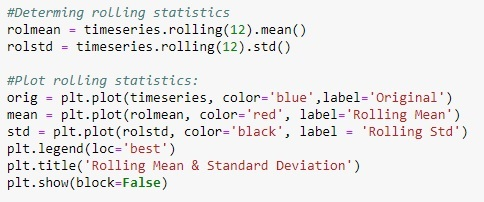
\includegraphics[width=\linewidth]{figures/fig-1-6-func.jpg}	
				\captionof{figure}{Notations}
				\label{fig: Notations}
				\end{center}

The function used for computing and plotting the figure 1.9 is as follows:\\

				\begin{center}
				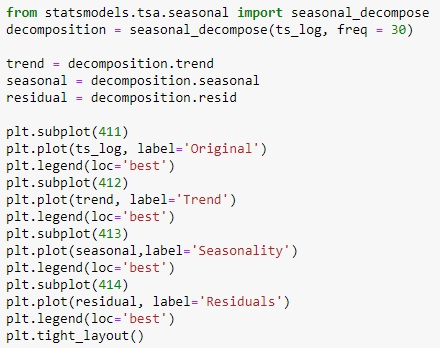
\includegraphics[width=\linewidth]{figures/fig-1-9-func.jpg}	
				\captionof{figure}{Notations}
				\label{fig: Notations}
				\end{center}
%\end{appendix}

Setup for Section 4.3:\\

URL : {https://colab.research.google.com/}
\begin{itemize}
\item[1.] Log on to the above url and you will be asked to create a file with python 3 or python 2 environment. 
\item[2.] GO to Edit-> Notebook Settings and select hardware accelerator as GPU.
\item[3.] Connect to the cloud environment by clicking on the connect button on top right corner of the page.
\item[4.] After got connected we are good to go.
\item[5.] Type your code, build your models and run it.
\end{itemize}



